\section{Komunikace \g{MS}}\label{sec:msa-communication}

Mikroslužby jsou definované jako vždy oddělené z hlediska procesů a pro komunikaci s jinými službami nebo externími systémy musí udržovat kompatibilní \g{API} vůči jejich rozhraní a prostředí.
U takové komunikace můžeme zkoumat typ, technologii a hierarchii/strukturu, jež se řídí požadavkami na systém.



\subsection{Typ komunikace}\label{subsec:msa-communication-type}
Typ komunikace se abstrahuje od konkrétních řešení a zkoumá pouze konceptuální potřeby komunikace systému.
Obecně se uvádí dělení na dvě podskupiny – dle počtu cílových služeb a dle synchronity komunikace, které se dají různě kombinovat, přícemž každá kombinace může mít víc podtypů~\cite{msachris}.
Celý přehled je uveden v následujícím seznamu:


\begin{dl}
   \item [Synchronní 1:1] – synchronní komunikace dvou subjektů.

   \begin{ul}
      \item \textbf{Dotaz/odpověď} – producent vytváří právě jeden dotaz na jinou službu a čeká na pozitivní, nebo negativní odpověď.
      Tento způsob vede ke zvýšení provázanosti \g{MS}.
   \end{ul}

   \item [Synchronní 1:N] – synchronní komunikace s více cíli nemůže existovat, protože by vznikla sekvence synchronních požadavků 1:1 kvůli jednomu producentu.

   \item [Asynchronní 1:1] – asynchronní komunikace dvou subjektů.

   \begin{ul}
      \item \textbf{Asynchronní dotaz/odpověď} – producent vytváří jeden dotaz a nečeká na okamžitou odpověď.
      Odpověď se může poskytnout kdykoliv (nebo vůbec) – chování nesmí být blokujícího typu.
      \item \textbf{Oznámení} – producent vytváří jeden dotaz (oznámení), zpětná komunikace se neočekává a neexistuje.
   \end{ul}

   \item [Asynchronní 1:N] – asynchronní komunikace s více cíli.

   \begin{ul}
      \item \textbf{Producent/konzument} – producent vytváří jeden dotaz a předává všem konzumentům.
      \item \textbf{Producent / asynchronní odpovědi} – producent vytváří jeden dotaz a poředává všem konzumentům.
      Následně čeká předem danou dobu na potenciální asynchronní odpovědi od konzumentů.
   \end{ul}
\end{dl}



\subsection{Technologie komunikace}\label{subsec:msa-communication-technology}
Technologií může být myšlen protokol nebo systém doporučení, která mohou být uplatněna v konkrétním programovacím jazyce.
Vzhledem k Node.js se může jednat například o následující způsoby:

\begin{dl}
   \item [REST] – běžné GET/POST/\ldots dotazy přes \g{HTTP}.
   \item [GraphQL] – dotazovací jazyk nad strukturovanými daty~\cite{graphql}.
   \item [gRPC] – framework založený na \g{RPC} protokolu~\cite{grpc}.
   \item [RabbitMq] – broker zpráv~\cite{rabbitmq}.
   \item [Kafka] – platforma pro distribuované streamování událostí~\cite{kafka}.
   \item [MQTT] – standard pro \g{IoT} komunikace~\cite{mqtt}.
\end{dl}

Výběr technologie má dopad na provázanost služeb v systému.
V případě například \g{REST} implementace bude provázanost větší kvůli požadovné odpovědi v relativně krátké době.
Volba RabbitMq naopak může zajistit menší provázanost tím, že zpracování se bude řídit brokerem zpráv, avšak v případě nutné okamžité odpovědi může způsobovat komplikace.


\subsection{Struktura komunikace}\label{subsec:msa-communication-structure}

Pokud pomineme konkrétní způsob výměny informací mezi mikroslužbami a podíváme na se obecnou organizaci komunikace, tak existují dva základní způsoby – orchestrace a choreografie~\cite{choreovsorch}.


\begin{dl}
   \item [Orchestrace] – předpokládá analogii s hudebním orchestrem, kdy každý člen systému zná vlastní roli, ale stejně musí být řízen dirigentem.
   V tomto případě dirigent je zastoupen orchestrační mikroslužbou, která vystupuje jako prvek, jenž zprostředkovává veškerou komunikaci.
   Tento koncept je úzce spjat s RESTful \g{API} a může v případě obrovského počtu \g{MS} způsobovat komplikace, protože orchestrační prvek bude muset zvládat stovky až tisíce mikroslužeb a ve výsledku dopadne jako těžce spravovatelná monolitická část~\cite{choreovsorch}.
   Z implementačního pohledu však může být o něco jednodušší, protože jakákoliv propagace chyb, sběr dat a další požadavky mohou být přímočářejší a soustředěny na jednom místě.

   \item [Choreografie] – analogicky představuje taneční skupinu, kde neexistuje řídící prvek, ale každý člen reaguje na podnět (hudbu, jiné členy) a provádí potřebné kroky.
   Implementacně musí existovat komunikace řízená událostmi, kdy jedna služba vysílá zprávu do brokera a o zbytek se nemusí starat, vše je řízeno asynchronně.
   Zárověň každá služba odposlouchává pouze zprávy, na které má reágovat.
   Tento koncept zajišťuje mnohem větší ohebnost a menší provázanost služeb~\cite{choreovsorch}.
   Přináší však potřebu lépe zpracovávat chyby kvůli asynchronním akcím, které nemusí nikdy doběhnout.
   Zejména se to projevuje u původně sycnhronních požadavků, například ze strany prohlížeče, kdy se musí čekat na odpověd.
   Aby nenastalo potenciálně nekonečné očekávání dokončení požadavku na server, tak se může zvolit přiměřeně dlouhá časová doba, kdy na straně serveru se vykonávání požadavku začne brát jako nezdařilé.
   V tomto případě se vrací chybná odpověd a je potřeba zrušit všechny změny, které byly provedené dosud a které se mohou provést po dokončení pomalu zpracovaného požadavku.
\end{dl}

Možná vizualizace obou struktur je znázorněna na obrázku~\ref{fig:msa-structure-communication}.
Samozřejmě může docházet i k prolínání takových řešení – například choreografie se sychnronní komunikací.


\begin{figure}[htbp]
   \centering
   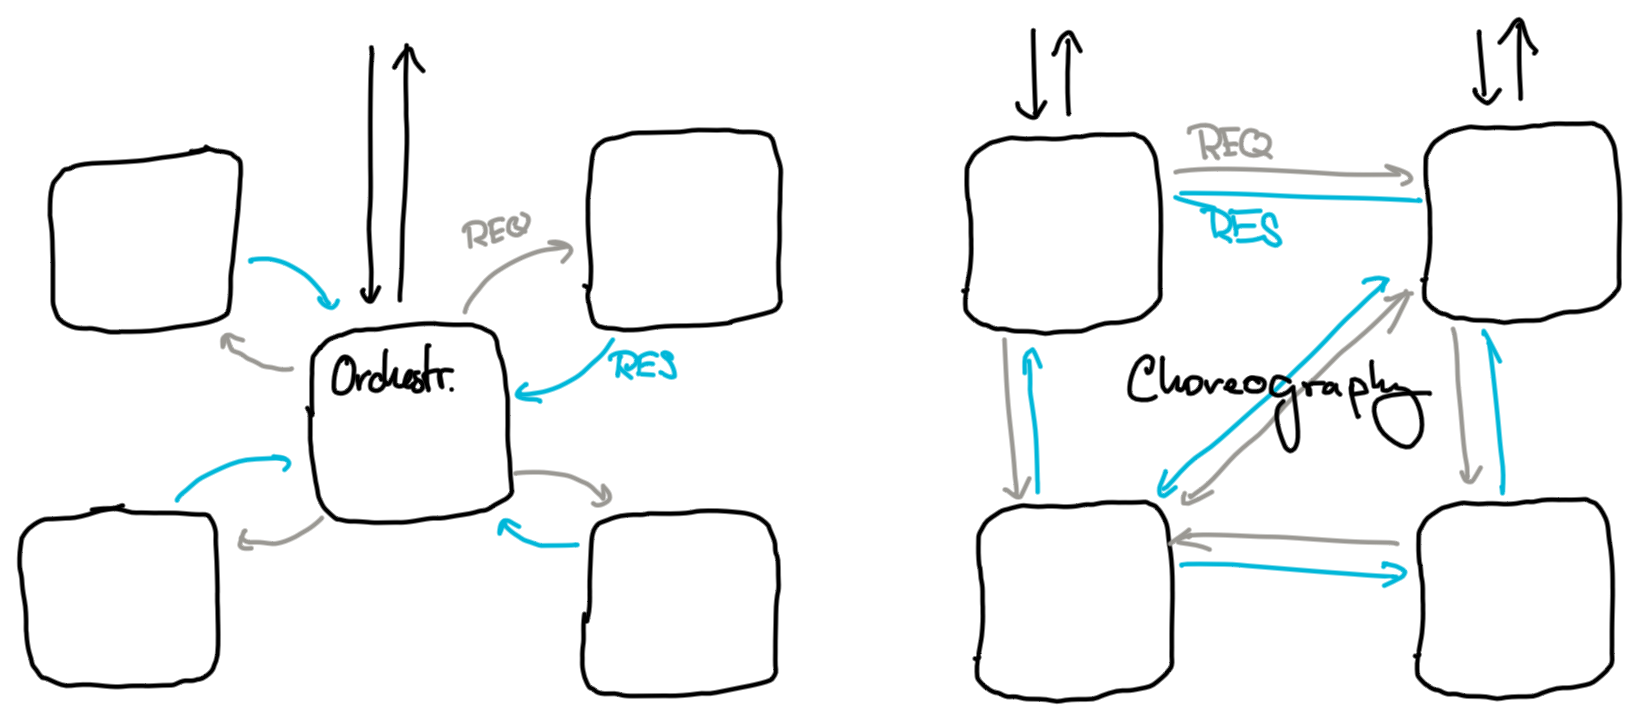
\includegraphics[max width=\textwidth]{assets/draft-msa-communication}
   \caption{Orchestrace a choreografie \g{MS}}\label{fig:msa-structure-communication}
\end{figure}



\section{Udržování závislostí}\label{sec:msa-dependencies}

V průběhu života systému a dodávaných řešení s \g{MSA} je pravděpodobné, že vlivem měnících se podmínek bude docházet i ke změnám potřeb poskytovaných rozhraní.
Takové modifikace mohou vést k nekonzistenci a narušení systému jako celku.
Tuto situaci je možné kontrolovat a řešit s pomocí sémantického verzování v různých variantách.


\subsection{Verzování v \g{URI}}\label{subsec:msa-dependencies-uri}

Zápis verze v \g{URI} může vypadat následovně:

\h{schema://domain/name-service/v1.0.0/entity}

Výhody:
\begin{ul}
   \item Je možné udržovat víc aktivních \g{API} verzí v rámci jedné \g{MS}.
   \item
\end{ul}

Nevýhody:
\begin{ul}
   \item V případě pevné vazby na verzi pro klientskou aplikaci může být nákladné sledovat aktualizace \h{minor} nebo \h{patch} verzí.
   Toto může být řešeno redukcí pouze na \h{major} verze (\h{.../v1/...}).
\end{ul}


\subsection{Verzování v hlavičkách \g{HTTP}}\label{subsec:msa-dependencies-headers}



\subsection{Verzování \g{MSA}}\label{subsec:msa-dependencies-msa}
Místo \g{API} je možné verzovat a hlídat samotné mikroslužby.
Výrazně se tím zkomplikuje možnost udržování několika poskytovaných rozhraní, protože každá verze bude vyžadovat vlastní adresu v rámci systému.
Na druhou stranu je možné u každé sluby definovat seznam závislostí, který by se poskytoval v rámci obecného dotazu ohledně stavu služby.
V případě existence konceptu registrace mikroslužby v systému by bylo možné tyto požadavky na závislosti kontrolovat a včas upozorňovat na nevhodnout sestavu mikroslužeb (viz obrázek~\ref{fig:version-reg}).


\begin{figure}[htbp]
   \centering
   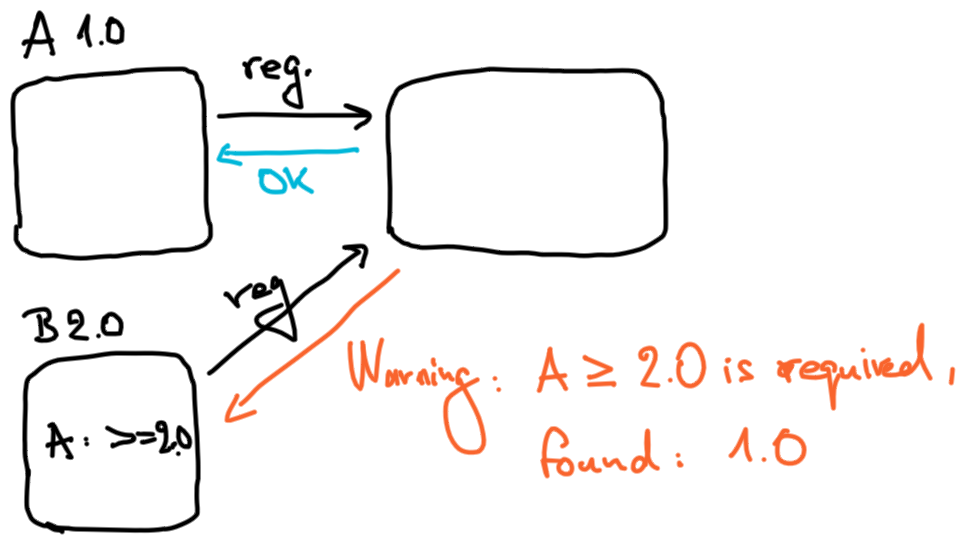
\includegraphics[max width=\textwidth]{assets/draft-version-reg}
   \caption{Registrace \g{MS} a kontrola závislostí}\label{fig:version-reg}
\end{figure}
